
\documentclass[8pt]{article}
%	options include 12pt or 11pt or 10pt
%	classes include article, report, book, letter, thesis

\usepackage[a4paper,bindingoffset=0.2in,%
            left=0.6in,right=0.6in,top=0.2in,bottom=0.4in,%
            footskip=.15in]{geometry}
            
\usepackage[T1]{fontenc}
\usepackage[polish]{babel}
\usepackage[utf8]{inputenc}
\usepackage{lmodern}
\selectlanguage{polish}
\usepackage{blindtext}
\usepackage{pgfplots}
\usepackage{graphicx}


\title{Algorytmy numeryczne}
\author{Zadanie 3 \\ Tomasz Adamczyk | Aleksander Kosma\\243217 | 238193\\grupa 1 tester-programista}
\date{13 Grudzień 2017}

\begin{document}
\maketitle 

\section*{Informacje wstępne}
Większość testów została przeprowadzona dla danych wejściowych:\\

\begin{center}
\begin{tabular}{  | c | c | c | }
  \hline
  rozmiar planszy & ilość grzybów & wartości kostki \\\hline
  7 &4& -4 -3 -2 -1 0 1 2 3 4\\\hline
   pozycje graczy & pozycje grzybów & prawdopodobieństwo kostki \\\hline
   3 4& 1 2 5 6& 1 1 1 1 1 1 1 1 1\\\hline
  \hline
\end{tabular} 
\end{center}


Weryfikacja poprawnego działania metody Monte Carlo. Tym więcej iteracji symulacji gry, tym wynik staje się precyzyjniejszy. W tym przypadku, wynik powinien zbiegać do wartości 0,6.
\begin{center}
 \makebox[\textwidth]{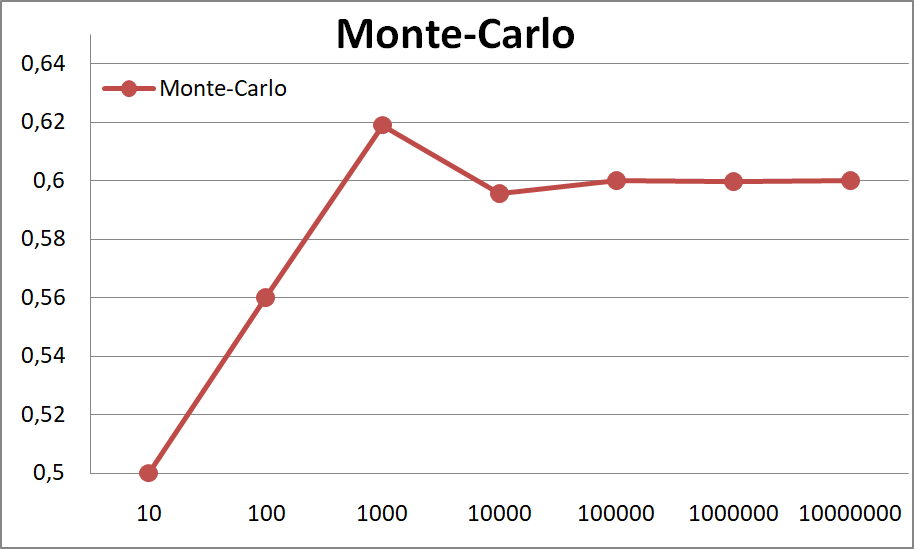
\includegraphics[width=10.5cm,height=6cm]{monte.png}}
\end{center}

\section*{Implementacja metod iteracyjnych}
W pierwszej części sprawozdania zbadamy poprawność metod iteracyjnych do rozwiązywania układów liniowych. Wyniki metod porównamy z wynikami Monte Carlo.\\
\begin{center}
\begin{tabular}{| p{3.2cm} | p{1.2cm}| p{2.2cm} | p{2.5cm} | p{2.5cm} | }
  \hline
  Rozmiar macierzy & Iteracje & Monte Carlo & Gauss Siedl & Jacobie \\\hline
  1598 &20&0,58998& 0,57727760827 & 0,57468277056 \\\hline
  1598 &50&0,58756& 0,58965872158 & 0,58952519470 \\\hline
  
  \hline
\end{tabular}
\end{center}
 .\\W przypadku kiedy ilość iteracji jest równa 20, różnica wyniku mieści się w granicy nawet ponad 1\% szansy na wygraną. W momencie kiedy iteracji jest już 50, różnica ta spada do zaledwie około 0.2\%.  Można więc stwierdzić, iż metody iteracyjne można wykorzystać do rozwiązania zagadnienia Grzybobranie.

\subsection*{Optymalna ilość iteracji w przypadku metod iteracyjnych}
Aby zoptymalizować czas potrzebny od wyliczenia wyniku przez metody iteracyjne, warto wiedzieć ile danych iteracji potrzebujemy. Stratą czasu jest liczenie kolejnego przybliżenia, które nic więcej nam nie powie. Za duża ilość iteracji może przeważyć na końcowych rezultatach i wnioskach.\\
Zastosowany został przez nas prosty algorytm, liczący średnią różnice sum wektora poprzedniego i aktualnego. Jeśli dana różnica jest mniejsza niż podany epsylon, kończymy kolejne iteracje. Dodatkowym zabezpieczeniem jest kontynuacja dopóki podana różnica jest mniejsza od epsylon określoną ilość z rzędu.\\
Wykres pokazuje mniejszą potrzebę iteracji dla Gaussa-Seidela. Jacobie potrzebuje więcej iteracji, jak i szybciej przyspiesza z kolejnymi wymaganymi iteracjami.
\begin{center}
 \makebox[\textwidth]{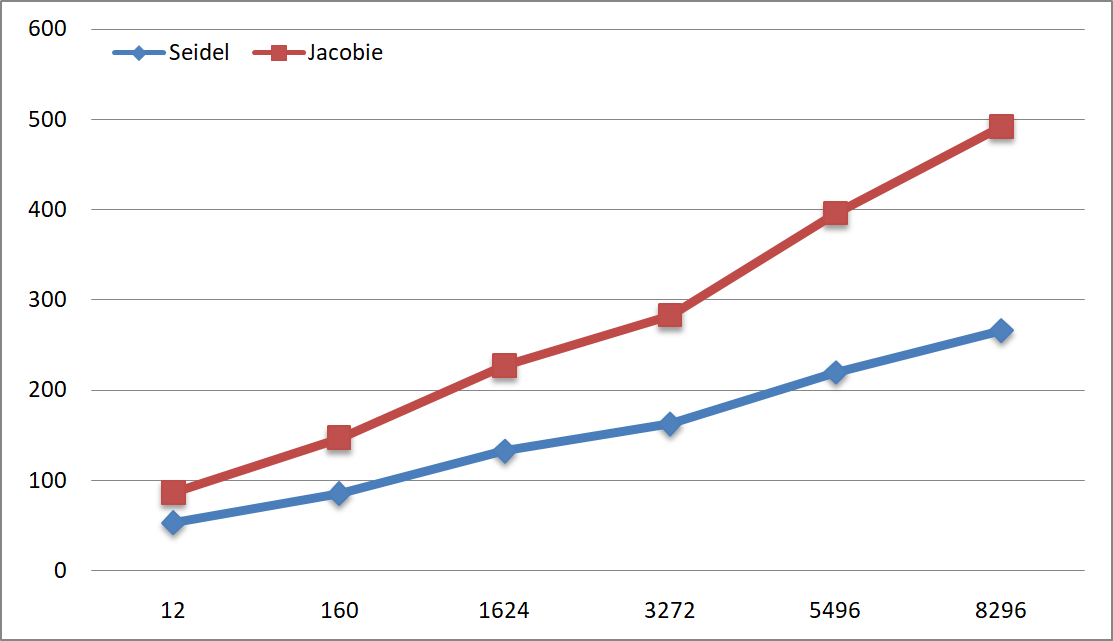
\includegraphics[width=12.5cm,height=7cm]{iteracje.png}}
\end{center}


\section*{Optymalny dobór metody w grze Grzybobranie}
Druga część opisuje wnioski, oparte o porównania wyników i czasu działania podanych metod:
\\\\
-metoda Gaussa z częściowym wyborem elementu podstawowego\\
-metoda Gaussa z częściowym wyborem elementu podstawowego z optymalizacją dla macierzy rzadkich\\
-metoda iteracyjna Gaussa-Seidela\\
-metoda iteracyjna Jacobiego\\
-metoda z biblioteki Eigen partialPivLu, z częściowym wyborem elemntu podstawowego\\
-metoda z biblioteki Eigen SparseLU, z częściowym wyborem przy użyciu macierzy rzadkich\\
\\
Poniższy wykres prezentuje czas potrzebny do rozwiązania równania. Eigen sprase ma miażdżącą przewagę nad resztą. Zdecydowanie najlepiej korzystać z tej metody. Jedynym jej mankamentem jest potrzeba dostarczenia wektora z informacją o ilości wartości miejsc niezerowych w kolumnach.
\begin{center}
 \makebox[\textwidth]{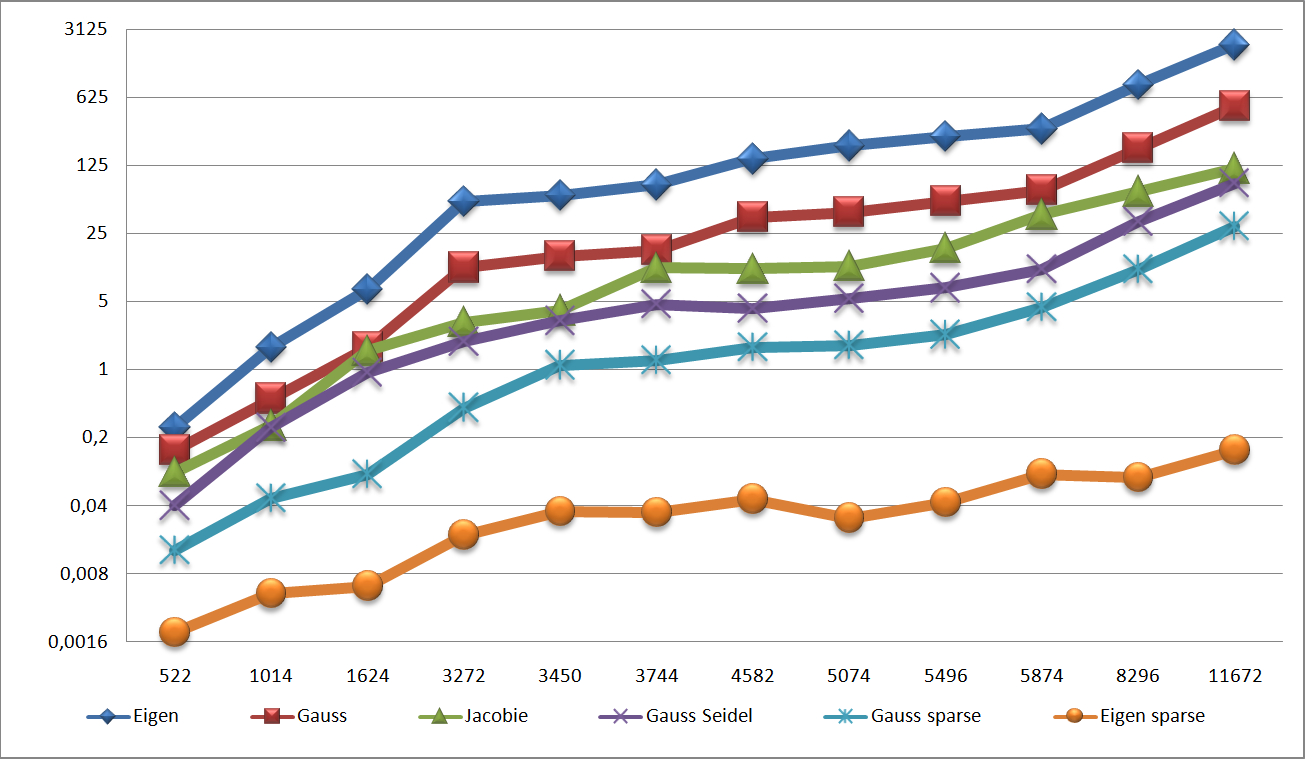
\includegraphics[width=17.5cm,height=10cm]{times.png}}
\end{center}
Precyzja wyników obliczona przez każdą z powyższych metod była praktycznie ta sama. W lwiej części sytuacji wyniki pokrywały się idealnie. Ma to związek z bardzo małą ilością wartości niezerowych. W konsekwencji komputer nie ma szansy zgubić gdzieś precyzji obliczeń. Prawdopodobnie wraz ze wzrostem macierzy, mogłyby się pojawić pewne różnice w wynikach.\\

Obliczenia wraz ze wzrostem rozmiaru macierzy były liczone od 10 do 2 próbek. Zazwyczaj tyle wystarczało by zauważyć tendencje. Wynik metody Monte Carlo do weryfikacji wyników, był obliczany każdorazowo dla miliona próbek.\\
\\
\begin{tabular}{ | p{8.2cm} | p{8.2cm} | }
  \hline
  \multicolumn{2}{|c|}{Podział obowiązków} \\
  \hline
  \multicolumn{1}{|c|}{\textbf{Aleksander Kosma} }& \multicolumn{1}{|c|}{\textbf{Tomasz Adamczyk}} \\
  \hline
  -Implementacja Monte Carlo & -Implementacja metod iteracyjnych \\\hline
   -Iteracyjne generowanie układu równań & -Ustalenie i implementacja warunków wygranej \\\hline
    -Szukanie gry bliskiej 50\% & -Wprowadzanie układu równań do macierzy \\\hline
  -Optymalizacja metod iteracyjnych i Gaussa & -Generowanie wyniku poprzez bibliotekę Eigen\\\hline
  -Testy i generowanie wyników & -Napisanie skryptów do generowania wyników \\\hline
  -Obróbka wyników, wykresy i opracowanie & - \\\hline
  
  \hline
\end{tabular}

\subsection*{Dodatkowo}

W momencie kiedy chcemy osiągnąć wynik jak najbardziej zbliżony do 50\% szans na wygraną, naszą intencją jest wydłużanie i  odwlekanie wygranej przez któregoś z graczy. W tym celu należy:\\
$\bullet$  \quad pozbyć się grzybów. Grzyby są ścieżką na skróty do wygrania. Określona ilość grzybów w rozgrywce, zdobyta wcześniej, od razu premiuje nas wygraną.\\
$\bullet$  \quad zmniejszyć kostkę do najmniejszych przeskoków. Najbardziej optymalna wersja to kostka ze ściankami o wartościach \{-1, 0 ,1\}. Zero na kostce jest kolejną szansą dla przeciwnika by odwrócić losy rozgrywki.\\
$\bullet$  \quad prawdopodobieństwo kostki powinno być jak największe dla zera.  W momencie kiedy zero wypada najczęściej, dynamika rozgrywki spada. Dzięki temu, któremuś z graczy trudniej stworzyć sobie szybką przewagę. \\
$\bullet$  \quad Ostatnią zmienną na którą mamy wpływ to pozycje startowe graczy. Znów chcemy by opóźnić wygraną, więc stawiamy obu graczy możliwie daleko od mety.\\
Najlepszy uzyskany wynik:  \textbf{0.5000000034688313}\\
\begin{center}
dane wejściowe: \\

\begin{tabular}{  | c | c | c | c | }
  \hline
  rozmiar planszy &pozycje startowe& wartości kostki & prawdopodobieństwo \\\hline
   101 & 50, 51  & -1, 0, 1& 1, 100000, 1\\\hline
  \hline
\end{tabular} 
\end{center}

\end{document}